
In this section, we remain in the classical realm. We introduce the standard subset-sum notations and heuristics and give a new presentation of the HGJ algorithm, putting an emphasis on the \emph{merge-and-filter} operation. We introduce our extended $\{-1,0,1,2\}$ representations and detail our improvements over BCJ.


\subsection{Notations and Conventions}

%\YS{Add Random Subset Sum Definition and the definition of $\negl$} \AS{check please}

Hereafter and in the rest of the paper, all time and memory complexities, classical and quantum, are exponential in $n$. We use the soft-O notation $\widetilde{\mathcal{O}}$ which removes polynomial factors in $n$, and focus on the asymptotic exponent, relative to $n$. We use $\negl(n)$ for any function that vanishes inverse-exponentially in $n$. We often replace asymptotic exponential time and memory complexities (\emph{e.g.} $\bigOt{2^{\alpha n}}$) by their exponents (\emph{e.g.} $\alpha$). We use capital letters (\emph{e.g.} $L$) and corresponding letters (\emph{e.g.} $\ell$) to denote the same value, in $\log_2$ and relatively to $n$: $\ell = \log_2(L) / n$. %In general, time and memory complexities will be replaced by their exponents.

\begin{definition}[Entropies and multinomial functions]
We define the following functions:
 \begin{enumerate}[topsep=0pt,leftmargin=3.6cm]
  \item[\bf Hamming Entropy:]$\entr{x} = - x \log_2 x - (1-x) \log_2 (1-x)$
  \item[\bf Binomial:]$\bin{\omega}{\alpha}  = \entr{\alpha / \omega} \omega$
  \item[\bf 2-way Entropy:]$g(x,y) = -x \log_2 x - y \log_2 y - (1-x-y) \log_2 (1-x-y)$
  \item[\bf Trinomial:]$\trin{\omega}{\alpha}{\beta} = g(\alpha / \omega, \beta / \omega) \omega$
  \item[\bf 3-way Entropy:]$f(x, y, z) =  - x \log_2 x - y \log_2 y - z \log_2 z -$\\
  \phantom{a} \hfill $(1-x-y-z) \log_2 (1-x-y-z)$
  \item[\bf Quadrinomial:] $\quadrin{\omega}{\alpha}{\beta}{\gamma} = f(\alpha/\omega, \beta/\omega, \gamma/\omega)\omega$
 \end{enumerate}
\end{definition}


\begin{property}[Standard approximations]%
 We have the following approximations, asymptotically in $n$:
\begin{center}$\bin{\omega}{\alpha} \simeq \frac{1}{n} \log_2{\omega n \choose \alpha n} ~~;~~ \trin{\omega}{\alpha}{\beta} \simeq \frac{1}{n} \log_2{\omega n \choose \alpha n, \beta n} $ $ \quadrin{\omega}{\alpha}{\beta}{\gamma} \simeq \frac{1}{n} \log_2 { \omega n \choose \alpha n, \beta n, \gamma n }$
\end{center}

\end{property}

% We denote by $\entr{x}$ the Hamming entropy of $x$: $\entr{x} = - x \log_2 x - (1-x) \log_2 (1-x)$. We use the standard approximation ${\alpha n \choose \beta n} \simeq 2^{\entr{\beta / \alpha} \alpha n}$, and we denote . % and write all (time and memory) complexities in $\log_2$.
% We also denote by $g$ the function: $g(x,y) = -x \log_2 x - y \log_2 y - (1-x-y) \log_2 (1-x-y)$. Then we have the approximation ${\alpha n \choose \beta n, \gamma n} \simeq 2^{g(\beta / \alpha, \gamma / \alpha) \alpha n}$, and we denote $\trin{\alpha}{\beta}{\gamma} = g(\beta / \alpha, \gamma / \alpha) \alpha n$.
% Finally, we denote by $f$ the function: $f(x, y, z) =  - x \log_2 x - y \log_2 y - z \log_2 y - (1-x-y-z) \log_2 (1-x-y-z)$, and $\quadrin{\omega}{\alpha}{\beta}{\gamma} = f(\alpha/\omega, \beta/\omega, \gamma/\omega)\omega n \simeq \log_2 { \omega n \choose \alpha n, \beta n, \gamma n }$
% 

\begin{definition}[Distributions of knapsacks]
A \emph{knapsack} or \emph{subknapsack} is a vector $\vec{e} \in \zomd^n$. The set of $\vec{e}$ with $\alpha n$ ``-1'', $(\alpha + \beta - 2\gamma) n$ ``1'', $\gamma n$ ``2'' and $(1 - 2\alpha - \beta + \gamma)n$ ``0'' is denoted $D^n[\alpha, \beta, \gamma]$. 
%We note $X^n[\alpha, \beta, \gamma]$ the random variable sampled uniformly in $D^n[\alpha, \beta, \gamma]$. 
If $\gamma = 0$, we may omit the third parameter. This coincides with the notation $D^n[\alpha, \beta]$ from~\cite{DBLP:conf/tqc/HelmM18}.
\end{definition}

Note that we always add vectors \emph{over the integers}, and thus, the sum of two vectors of $D^n[*,*,*]$ may contain unwanted symbols $-2, 3$ or $4$.

\begin{property}[Size of knapsack sets]
\label{property:knapsack_size}
We have:
\begin{center}
$\frac{1}{n} \log_2 | D^n[0, \beta,0] | \simeq h(\beta) ~~; ~~\frac{1}{n} \log_2 | D^n[\alpha, \beta, 0] | \simeq  g(\alpha, \alpha + \beta)$
\vspace{1em}

$ \frac{1}{n} \log_2 | D^n[\alpha, \beta, \gamma] | \simeq f(\alpha, \alpha + \beta - 2\gamma, \gamma) \enspace. $
\end{center}



\end{property}


\paragraph{Subset-sum.}The problem we will solve is defined as follows:
\begin{definition}[Random subset-sum instance of weight {$n/2$}]
Let $\vec{a}$ be chosen uniformly at random from $\left(\mathbb{Z}_{N}\right)^n$, where $N \simeq 2^n$. Let $\vec{e}$ be chosen uniformly at random from $D^n[0, 1/2, 0]$. Let $t = \vec{a} \cdot \vec{e} \pmod{N}$. Then $(\vec{a}, t)$ is a \emph{random subset-sum instance}. A \emph{solution} is a vector $\vec{e'}$ such that $\vec{a} \cdot \vec{e'} = t \pmod{N}$.
\end{definition}

%\paragraph{Distributions.}
%We reuse the notation $D^n[\alpha, \beta]$ from~\cite{DBLP:conf/tqc/HelmM18} to denote the set of vectors $\vec{e} \in \zom^n$ with $\alpha n$ ``$-1$'', $(\alpha + \beta) n$ ``1'' and $(1 - 2\alpha -  \beta)n$ ``0''. We will often consider subknapsacks taken uniformly at random from $D^n[\alpha, \beta]$, and use a corresponding random variable $X^n[\alpha, \beta]$.

\paragraph{Sampling.}
Throughout this paper, we assume that we can classically sample uniformly at random from $D^n[\alpha, \beta, \gamma]$ in time $\poly(n)$. (Since $\alpha n$, $\beta n$ and $\gamma n$ will in general not be integer, we suppose to have them rounded to the nearest integer.)
%, and proceed with $\alpha n$, $\beta n$ and $\gamma n$ as if they were integers. 
This comes from an efficient bijection between representations and integers (see \ifeprint Appendix~A\else Appendix A in the full version of the paper~\cite{DBLP:journals/iacr/BonnetainBSS20}\fi).
% (see Lemma~\ref{lemma:representation-bijection} in \ifeprint Appendix \else Supplementary Material \fi ~\ref{appendix:rpbijection}). 
In addition, we can efficiently produce the uniform superposition of vectors of $D^n[\alpha, \beta, \gamma]$, using $\poly(n)$ quantum gates, and we can perform a quantum search among representations.


%\AS{Ça ne doit pas être vrai en général : toutes les paires en sortie n'ont pas la même probabilité de se faire jeter.}

%In other words, the setting of the modular constraint does not influence the distribution of weights in the subknapsack. %Another version of this heuristic appears e.g. in \AS{TQC18, but please check, this should indeed be equivalent}, in the sense that all pairs of vectors summed during the algorithm remain independent.

%\AS{we may not have spoken of lists yet. Move this elsewhere? Also, quoting TQC18}
%This heuristic allows to show, by a Chernoff bound, that the actual list sizes are close to their expectation. When a knapsack instance $\vec{a}$ is drawn uniformly at random, then for all lists $L$ in the algorithm, $|L| = \bigO{\mathbb{E}(|L|)}$ with a probability exponentially close to one in $n$.

\subsection{Merging and Filtering}
\label{subsection:merging-filtering}

In all subset-sum algorithms studied in this paper, we repeatedly sample vectors with certain distributions $D^n[*, *, *]$, then combine them. Let $D_1 = D^n[\alpha_1, \beta_1, \gamma_1]$, $D_2 = D^n[\alpha_2, \beta_2, \gamma_2]$ be two input distributions and $D = D^n[\alpha, \beta, \gamma]$ be a target. Given two lists $L_1 \in D_1^{|L_1|}$ and $L_2 \in D_2^{|L_2|}$, we define:
%, then find pairs of such vectors $\vec{e}_1, \vec{e}_2 \in D_1 \times D_2$ such that: 1) $(\vec{e}_1 + \vec{e}_2) \cdot \vec{a} = t \mod{M}$ for some integers $t$ and $M$; 2) $\vec{e}_1 + \vec{e}_2$ belongs to a target distribution $D = D^n[\alpha, \beta, \gamma]$. Let $L_1 \subseteq D_1^{|L_1|}$ and $L_2 \subseteq D_2^{|L_2|}$, then we define:
\begin{itemize}
\item the \emph{merged list} $L = L_1 \bowtie_c L_2$ containing all vectors $\vec{e} = \vec{e_1} + \vec{e_2}$ such that: $\vec{e_1} \in L_1, \vec{e_2} \in L_2$, $(\vec{e}_1 + \vec{e}_2) \cdot \vec{a} = s \mod{M}$, $s \leq M$ is an arbitrary integer and $M \approx 2^{cn}$ (we write $L_1 \bowtie_c L_2$ because $s$ is an arbitrary value, whose choice is without incidence on the algorithm)
\item the \emph{filtered list} $L^f = (L \cap D) \subseteq L$, containing the vectors with the target distribution of $1, -1, 2$ (the target $D$ will always be clear from context).
\end{itemize}
In general, $L$ is exponentially bigger than $L^f$ and does not need to be written down, as vectors can be filtered on the fly. The algorithms then repeat the merge-and-filter operation on multiple levels, moving towards the distribution $D^n[0, 1/2]$ while increasing the bit-length of the modular constraint, until we satisfy $\vec{e} \cdot \vec{a} = t \mod{2^n}$ and obtain a solution. Note that this merging-and-filtering view that we adopt, where the merged list is repeatedly sampled before an element passes the filter, has some similarities with the ideas developed in the withdrawn article~\cite{DBLP:journals/corr/abs-1907-04295}.


The standard subset-sum heuristic assumes that vectors in $L^f$ are drawn independently, uniformly at random from $D$. It simplifies the complexity analysis of both classical and quantum algorithms studied in this paper. Note that this heuristic, which is backed by experiments, actually leads to provable probabilistic algorithms in the classical setting (see~\cite[Theorem 2]{DBLP:conf/eurocrypt/BeckerCJ11}). We adopt the version of~\cite{DBLP:conf/tqc/HelmM18}.

\begin{heuristic}
\label{heur1}
If input vectors are uniformly distributed in $D_1 \times D_2$, then the filtered pairs are uniformly distributed in $D$ (more precisely, among the subset of vectors in $D$ satisfying the modular condition).
\end{heuristic}

\paragraph{Filtering Representations.} We note $\ell = (1/n)\log_2|L|$, and so on for $\ell_1, \ell_2, \ell^f$.
By Heuristic~\ref{heur1}, the average sizes of $L_1$, $L_2$, $L$ and $L^f$ are related by:
\begin{itemize}
\item $\ell = \ell_1 + \ell_2 - c$
\item $\ell^f = \ell + \pf$, where $\pf$ is negative and $2^{\pf n}$ is the probability that a pair $(\vec{e_1}, \vec{e_2})$, drawn uniformly at random from $D_1 \times D_2$, has $(\vec{e_1} + \vec{e_2}) \in D$.
\end{itemize}
In particular, the occurrence of collisions in $L^f$ is a negligible phenomenon, unless $\ell^f$ approaches ($\log_2 |D| / n) - c$, which is the maximum number of vectors in $D$ with constraint $c$. For a given random knapsack problem, with high probability, the size of any list built by sampling, merging and filtering remains very close to its average (by a Chernoff bound and a union bound on all lists).

Here, $\pf$ depends only on $D_1, D_2$ and $D$. Working with this \emph{filtering probability} is especially useful for writing down our algorithm in Section~\ref{section:hgj-asymmetric}. We give its formula for $\zo$ representations below. Two similar results for $\zom$ and $\zomd$ can be found in \ifeprint Appendix\else the full version of the paper~\cite{DBLP:journals/iacr/BonnetainBSS20}\fi.

%\ifeprint Appendix\else Supplementary Material\fi~\ref{appendix:filter}.


\begin{lemma}[Filtering HGJ-style representations]
\label{lemma:hgj-filter}
Let $\vec{e_1} \in D^n[0, \alpha]$ and $\vec{e_2} \in D^n[0, \beta]$ be drawn uniformly at random. The probability that $\vec{e_1} + \vec{e_2} \in D^n[0, \alpha + \beta]$ is $0$ if $\alpha + \beta > 1$, and $2^{\pfilterhgj{\alpha}{\beta}n}$ otherwise, with 
$$\pfilterhgj{\alpha}{\beta} = \bin{1-\alpha}{\beta} - \entr{\beta} = \bin{1-\beta}{\alpha} - \entr{\alpha} \enspace.$$
%if $\alpha + \beta \leq 1$, and the probability is $0$ otherwise.
\end{lemma}

\begin{proof}
The probability that a $\vec{e}_1 + \vec{e}_2$ survives the filtering is:
$$ {n - \alpha n \choose \beta n} / {n \choose \beta n} = {n - \beta n \choose \alpha n} / {n \choose \alpha n} \enspace.$$
Indeed, given a choice of $\alpha n$ bit positions among $n$, the other $\beta n$ bit positions must be compatible, hence chosen among the $(1-\alpha)n$ remaining positions. By taking the $\log_2$, we obtain the formula for the filtering probability. \qed
%$$ \bin{1-\alpha}{\beta} - \entr{\beta} = \bin{1-\beta}{\alpha} - \entr{\alpha} \enspace.$$
\end{proof}


%\paragraph{Size of Filtered Lists.}
%\AS{check if we really use that in the proba computation. I'm not sure.}
%Our complexity analyses are average-case, but list sizes deviate only negligibly from their expectation, as the following Lemma shows.

%Assume that we merge two lists $L_1$ of size $\ell_1$ and $L_2$ of size $\ell_2$ (in $\log_2$, and in multiple of $n$), with a modular constraint on $c$ bits, and a filtering probability (either with HGJ- or BCJ-style representations) $p$ given by the previous lemmas. Let $L = L_1 \bowtie_c L_2$ be the merged list and $L^f$ the filtered list. Then notice that the expected sizes of $L$ and $L^f$ are related by $\mathbb{E}(|L^f|) = 2^{pn} \mathbb{E}(|L|)$. We have the following lemma.

%\begin{lemma}%\label{lemma:chernoff}
%Assuming Heuristic~\ref{heur1}, assuming that $|L_1|, |L_2|, |L^f|$ are exponential in $n$, there exists a constant $r$ such that, with probability $1 - e^{-r n}$ on the subset-sum instance:
%$$ \frac{1}{2} \mathbb{E}(|L^f|) \leq |L^f| \leq 2 \mathbb{E}(|L^f|) \text{ and } \frac{1}{2} \mathbb{E}(|L|) \leq |L| \leq 2 \mathbb{E}(|L|) \enspace.$$
%\end{lemma}
%
%\begin{proof}
%By Heuristic~\ref{heur1}, each of the pairs $\vec{e_1}, \vec{e_2} \in L_1 \times L_2$ will fall in $L$ independently, with a constant probability. Hence, $|L|$ (resp. $|L^f|$) is a random variable which is the sum of $|L|$ (resp. $|L^f|$) independent random variables, and we can use an additive Chernoff bound: $ \Prob{}{ |L| \geq 2 \mathbb{E}(|L|) } \leq e^{ -2 \mathbb{E}(|L|) / 3 } $ and $ \Prob{}{ |L| \leq \frac{1}{2} \mathbb{E}(|L|) } \leq e^{ - \mathbb{E}(|L|) / 8 }$. Since $\mathbb{E}(|L|)$ is exponential in $n$, we can crudely bound it by a linear function in $n$. \qed
%\end{proof}

%Assume furthermore that the elements in $|L|$ are subknapsacks $\vec{e} \in D^n[\alpha, \beta]$ with a modular constraint $d$. Then, up to a polynomial factor in $n$, the expected size of $L^f$ is $\min \left( (\ell_1 + \ell_2 -c + p), g(\alpha, \beta) - d \right)$. Indeed, there are $2^{n (\ell_1 + \ell_2)}$ pairs, that we assume independent. They pass the modular constraint with probability $2^{-nc}$ and the filter with probability polynomially close to $2^{np}$. The filtered vectors are uniformly random in $D^n[\alpha, \beta]$. Hence collisions between them are negligible until the output list becomes \emph{saturated}, that is, it reaches its maximal size $g(\alpha, \beta) - d$ (the total number of subknapsacks with this modular constraint).

\paragraph{Time Complexity of Merging.}
Classically, the time complexity of the merge-and-filter operation is related to the size of the \emph{merged list}.

\begin{lemma}[Classical merging with filtering]
\label{lemma:classical-merging}
Let $L_1$ and $L_2$ be two sorted lists stored in classical memory with random access. 
In $\log_2$, relatively to $n$, and discarding logarithmic factors, merging and filtering $L_1$ and $L_2$ costs a time $\max( \min(\ell_1, \ell_2), \ell_1 + \ell_2 - c )$ and memory $\max( \ell_1, \ell_2, \ell^f)$, assuming that we must store the filtered output list.
%Then the filtered list $L_1 \bowtie_c^f L_2$, with a $nc$-bit modular condition, and a filtering probability $\pf$, can be written in time: 
%$$ \max \left( \min( |L_1|, |L_2|), \frac{|L_1 | |L_2|}{2^{nc}} \right) \enspace.$$
\end{lemma}

\begin{proof}Assuming sorted lists, there are two symmetric ways to produce a stream of elements of $L_1 \bowtie_c L_2$: we can go through the elements of $L_1$, and for each one, find the matching elements in $L_2$ by dichotomy search (time $\ell_1 + \max(0, \ell_2 - c)$) or we can exchange the role of $L_1$ and $L_2$. Although we do not need to store $L_1 \bowtie_c L_2$, we need to examine all its elements in order to filter them.\qed
\end{proof}
%

\subsection{Correctness of the Algorithms}

While the operation of \emph{merging and filtering} is the same as in previous works, our complexity analysis differs~\cite{DBLP:conf/eurocrypt/Howgrave-GrahamJ10,DBLP:conf/eurocrypt/BeckerCJ11,DBLP:conf/pqcrypto/BernsteinJLM13,DBLP:conf/tqc/HelmM18}. We enforce the constraint that the final list contains a single solution, hence if it is of size $2^{n \ell_0}$, we constrain $\ell_0 = 0$. Next, we limit the sizes of the lists so that they do not contain duplicate vectors: these are \emph{saturation constraints}. A list of size $2^{n \ell}$, of vectors sampled from a distribution $D$, with a constraint of $cn$ bits, has the constraint: $\ell \leq \frac{1}{n}\log_2{|D|} - c$. This says that there are not more than $|D| / 2^{cn}$ vectors $\vec{e}$ such that $\vec{e} \cdot \vec{a} = r \pmod{2^{cn}}$ for the (randomly chosen) arbitrary constraint $r$.

Previous works focus on the solution vector $\vec{e}$ and compute the number of \emph{representations} of $\vec{e}$, that is, the number of ways it can be decomposed as a sum: $\vec{e} = \vec{e}_1 + \ldots + \vec{e}_t$ of vectors satisfying the constraints on the distributions. Then, they compare this with the probability that a given representation passes the arbitrary constraints imposed by the algorithm. As their lists contains all the subknapsacks that fulfill the constraint, this really reflects the number of duplicates, and it suffices to enforce that the number of representations is equal to the inverse probability that a representation fulfills the constraint. If the two lists we merge are not of maximal size, the size of the merged list is the number of elements that fulfill the corresponding distribution times the probability that such an element is effectively the sum of two elements in the initial lists.

%For smaller lists, it suffices to add the probability that a representation compatible with the constraint is indeed in the list.

%\paragraph{Complexity Analysis.} The algorithms presented here are merging trees. We focus here on the asymptotic exponent, and dismiss the polynomial factors. To ensure the correctness of these algorithms, we make sure that on average, there is one solution at the end. This is not sufficient, and to avoid the cases where some instances have exponentially many solutions while most others have none, we limit the size of the lists such that they will not contain duplicates.

%\paragraph{Counting duplicates.} To compute the  number of duplicates of the solution $\vec{e}$, the previous works \cite{DBLP:conf/eurocrypt/Howgrave-GrahamJ10,DBLP:conf/eurocrypt/BeckerCJ11,DBLP:conf/pqcrypto/BernsteinJLM13,DBLP:conf/tqc/HelmM18} computed the \emph{number of representations} of the solution, that is, the number of ways it can be decomposed as a sum of subknapsacks that fulfil the distributions imposed by the algorithm, and compared it with the probability that a given representation passes the arbitrary constraints imposed by the algorithm. As their lists contains all the subknapsacks that fulfils the constraint, this really reflects the number of duplicates, and it suffices to enforce that the number of representations is equal to the inverse probability that a representation fulfils the constraint. For smaller lists, it suffices to add the probability that a representation compatible with the constraint is indeed in the list.

%We propose a slightly different approach. We compute for each step in the merging tree the probability that the sum of two subknapsacks passes the merging and filtering step, enforce that each list is smaller than its maximal size, and that the final list is of size 1.

The two approaches are strictly equivalent, as the probability that the sum of two subknapsacks is valid is exactly the number of representations of the sum, divided by the number of pairs of subknapsacks.

% 
% In the following we show that our approach is correct and is equivalent to the previous approach of counting representations. 
% 
% Let $D_1 = D^n[\alpha_1, \beta_1, \gamma_1]$, $D_2 = D^n[\alpha_2, \beta_2, \gamma_2]$ be two input distributions and $D = D^n[\alpha, \beta, \gamma]$ a target. Given two lists $L_1 \in D_1^{|L_1|}$ and $L_2 \in D_2^{|L_2|}$ where all vectors in $L_1$ and $L_2$ are uniformly drawn from $D_1$ and $D_2$, our constraints impose: $l_1+l_2-c+\pf\leq \frac{1}{n}\log_2{|D|}$. This implies: $c\geq l_1+l_2+\pf-\frac{1}{n}\log_2{|D|}$.
% The last term is exactly the nomber of times each vector $\vec{e}\in D $ is decomposed as a sum of $\vec{e_1}\in D_1$ and $\vec{e_2}\in D_2$. This inequality thus shows that by choosing an arbitrary $s \mod M$, at most a constant number of the same representation will appear in the filtered list $L^f$.
%as a complete solution is found if and only if its subknapsacks passes all the filtering steps

\subsection{The HGJ Algorithm}

We start our study of classical subset-sum by recalling the algorithm of Howgrave-Graham and Joux~\cite{DBLP:conf/eurocrypt/Howgrave-GrahamJ10}, with the corrected time complexity of~\cite{DBLP:conf/eurocrypt/BeckerCJ11}.
 %The basic operation in HGJ is to merge two lists of subknapsacks with a constraint $t$ on $c n$ bits, that is, from two lists $L_1$ and $L_2$, obtain the list $L' = \{ \vec{e}_1 + \vec{e}_2, \vec{e}_1 \in L_1, \vec{e}_2 \in L_2, (\vec{e}_1 + \vec{e}_2) \cdot \vec{a} = t \mod{2^{cn}} \}$. Furthermore, we are interested in the \emph{filtered} list of such representations, in which we remove duplicate representations and sums $\vec{e} = \vec{e}_1 + \vec{e}_2$ where $\vec{e}$ is not a binary vector. The length of the filtered list $L$ determines how many representations will survive the constraint $t$. In HGJ, all lists at a given level have the same size.
%\paragraph{The HGJ Algorithm.}
The algorithm builds a merging tree of lists of subknapsacks, with four levels, numbered $3$ down to $0$. Level $j$ contains $2^j$ lists. In total, $8$ lists are merged together into one.
\begin{description}
\item[Level 3.] We build 8 lists denoted $L_0^3 \ldots L_7^3$. They contain \emph{all} subknapsacks of weight $\frac{n}{16}$ on $\frac{n}{2}$ bits, either left or right:
\begin{align*}
\left\{ \begin{matrix}
L_{2i}^3 & = D^{n/2}[0, 1/8] \times \{ 0^{n/2} \} \\
L_{2i+1}^3 & =  \{ 0^{n/2} \} \times D^{n/2}[0, 1/8] 
\end{matrix} \right.
\end{align*}

%. We use a left-right split: for each pair $L_{2i}^3, L_{2i+1}^3$, the list $L_{2i}^3$ contains all subknapsacks $\vec{e}$ of Hamming weight $\frac{n}{16}$ on the left $\frac{n}{2}$ bits, and $0$ on the right $\frac{n}{2}$ bits, and the list $L_{2i+1}^3$ takes all subknapsacks on the other half. 
%This allows to avoid filtering when merging $L_{2i}^3$ and $L_{2i+1}^3$, since the positions set to 1 cannot interfere. 
From Property \ref{property:knapsack_size}, these level-3 lists have size $\ell_3 =  \entr{1/8} / 2$. As the positions set to 1 cannot interfere, these is no filtering when merging $L_{2i}^3$ and $L_{2i+1}^3$.
\item[Level 2.] We merge the lists pairwise with a (random) constraint on $c_2 n$ bits, and obtain 4 filtered lists. The size of the filtered lists plays a role in the memory complexity of the algorithm, but the time complexity depends on the size of the unfiltered lists.

In practice, when we say ``with a constraint on $c_j n$ bits'', we assume that given the subset-sum objective $t$ modulo $2^n$, random values $r_i^j$ such that $\sum_i r_i^j = t \mod{2^{c_jn}}$ are selected at level $j$, and the $r_i^j$ have $c_j n$ bits only. Hence, at this step, we have selected 4 integers on $c_2 n$ bits $r^1_0, r^1_1, r^1_2, r^1_3$ such that $r^1_0 + r^1_1 + r^1_2 + r^1_3 = t \mod{2^{c_2n}}$. The 4 level-2 lists $L_0^2, L_1^2, L_2^2, L_3^2$ have size $\ell_2 = (\entr{1/8} - c_2)$, they contain subknapsacks of weight $\frac{n}{8}$ on $n$ bits.

\begin{remark}
The precise values of these $r_i$ are irrelevant, since they cancel out each other in the end. They are selected at random during a run of the algorithm, and although there could be ``bad'' values of them that affect significantly the computation, this is not expected to happen.
\end{remark}

\item[Level 1.] We merge the lists pairwise with $(c_1 - c_2) n$ new bits of constraint, ensuring that the constraint is compatible with the previous ones. We obtain two filtered lists $L_0^1, L_1^1$, containing subknapsacks of weight $n/4$. They have size:
$$ \ell_1 = 2 \ell_2 - (c_1 - c_2) + \pfilterhgj{1/8}{1/8} $$
where $\pfilterhgj{1/8}{1/8}$ is given by Lemma~\ref{lemma:hgj-filter}.% = (1-1/8) \cdot \entr{1/8 / (1-1/8) } - \entr{1/8} =  7/8 \entr{1/7} - \entr{1/8} $.
%where $(1-1/8) \cdot \entr{1/8 / (1-1/8) } - \entr{1/8}$ is the filtering term.

\item[Level 0.] We find a solution to the subset-sum problem with the complete constraint on $n$ bits. This means that the list $L^0$ must have expected length $\ell_0 = 0$. Note that there remains $(1 - c_1) n$ bits of constraint to satisfy, and the filtering term is similar as before, so:
$$ \ell_0 = 2 \ell_1 - (1-c_1) + \pfilterhgj{1/4}{1/4} \enspace.$$%
%where $\pfilterhgj{1/4}{1/4} = (1-1/4) \cdot \entr{1/4 / (1-1/4) } - \entr{1/4}$.
\end{description}

\begin{figure}[htb]
\centering
\scalebox{0.75}{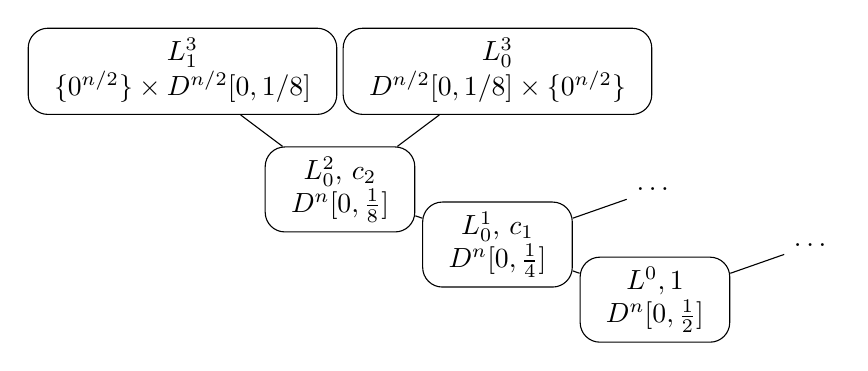
\begin{tikzpicture}[grow=up,nodes={draw,rectangle,rounded corners=.25cm,->}, level 1/.style={sibling distance=40mm, level distance=7mm}, level 2/.style={sibling distance=40mm}, level 3/.style={sibling distance=40mm, level distance=15mm}]
\node{ \begin{tabular}{c} $L^0, 1 $\\ $D^n[0, \frac{1}{2}]$ \end{tabular}}
	child { node[draw=none] {\dots }}
    child { node {\begin{tabular}{c} $L_0^1$, $c_1$ \\ $D^n[0, \frac{1}{4}]$ \end{tabular} }
    	child { node[draw=none] {\dots } }
    	child { node {\begin{tabular}{c} $L_0^2 $, $c_2$ \\ $D^n[0, \frac{1}{8}]$ \end{tabular} }
			child { node {\begin{tabular}{c} $L_0^3 $ \\ $D^{n/2}[0, 1/8] \times \{ 0^{n/2} \}$ \end{tabular} }}
			child { node {\begin{tabular}{c} $L_1^3 $ \\ $\{ 0^{n/2} \} \times D^{n/2}[0, 1/8] $ \end{tabular} }} }
    	};
\end{tikzpicture}}
\caption{The HGJ algorithm (duplicate lists are omitted)}
\label{fig:hgj-original}
\end{figure}

By Lemma~\ref{lemma:classical-merging}, the time complexity of this algorithm is determined by the sizes of the unfiltered lists:~~$ \max\left( \ell_3, 2\ell_3 - c_2, 2\ell_2 - (c_1 - c_2), 2 \ell_1 - (1-c_1) \right)$.

The memory complexity depends of the sizes of the filtered lists: $\max\left( \ell_3, \ell_2, \ell_1\right)$. By a numerical optimization, one obtains a time exponent of $0.337 n$.


\subsection{The BCJ Algorithm and our improvements}\label{subsection:new-classical-bcj}

The HGJ algorithm uses representations to increase artificially the search space. The algorithm of Becker, Coron and Joux~\cite{DBLP:conf/eurocrypt/BeckerCJ11} improves the runtime exponent down to $0.291$ by allowing even more freedom in the representations, which can now contain ``$-1$''s. The ``$-1$''s have to cancel out progressively, to ensure the validity of the final knapsack solution.

\begin{figure}[htb]
\centering
\scalebox{0.8}{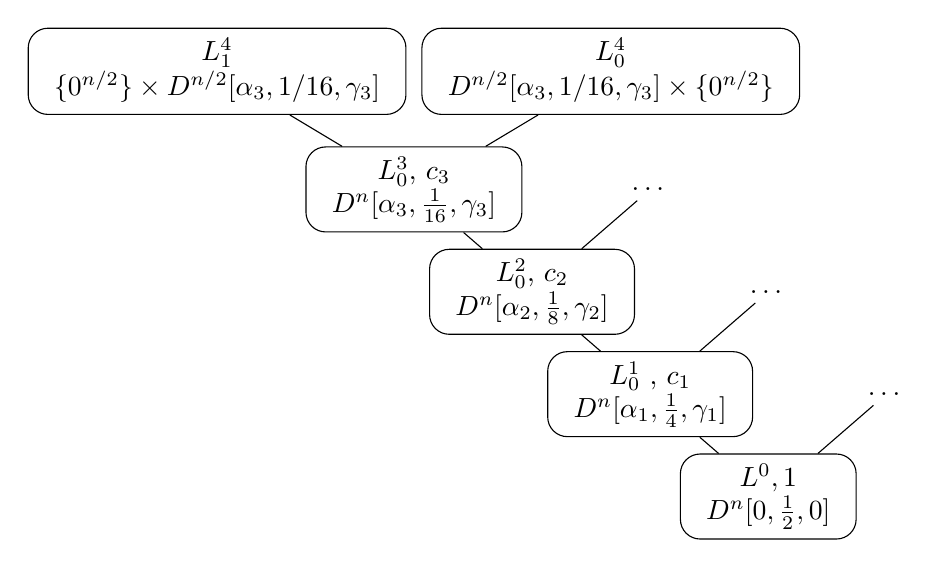
\begin{tikzpicture}[grow=up,nodes={draw,rectangle,rounded corners=.25cm,->}, level 1/.style={sibling distance=30mm, level distance=13mm}, level 2/.style={sibling distance=30mm}, level 3/.style={sibling distance=30mm}, level 4/.style={sibling distance=50mm, level distance=15mm}]
\node{ \begin{tabular}{c} $L^0, 1 $\\ $D^n[0, \frac{1}{2},0]$ \end{tabular}}
    child {node[draw=none] {\dots}}
    child { node {\begin{tabular}{c} $L_0^1$ , $c_1$ \\ $D^n[\alpha_1, \frac{1}{4}, \gamma_1]$ \end{tabular} }
    	child { node[draw=none] {\dots} }
    	child { node {\begin{tabular}{c} $L_0^2 $, $c_2$ \\ $D^n[\alpha_2, \frac{1}{8}, \gamma_2]$ \end{tabular} }
    		child { node[draw=none] {\dots}}
    		child { node {\begin{tabular}{c} $L_0^3 $,  $c_3$ \\ $D^n[\alpha_3, \frac{1}{16}, \gamma_3]$ \end{tabular} }
			child { node {\begin{tabular}{c} $L_0^4 $ \\ $D^{n/2}[\alpha_3, 1/16, \gamma_3] \times \{ 0^{n/2} \}$ \end{tabular} }}
			child { node {\begin{tabular}{c} $L_1^4 $ \\ $\{ 0^{n/2} \} \times D^{n/2}[\alpha_3, 1/16, \gamma_3] $ \end{tabular} }}
	}}};
\end{tikzpicture}}
\caption{Our improved algorithm (duplicate lists are omitted).}
\label{fig:bcj-original}
\end{figure}

We improve over this algorithm in two different ways. First, we relax the constraints $\ell_j + c_j = g(\alpha_j, 1/2^{j+1})$ enforced in~\cite{DBLP:conf/eurocrypt/BeckerCJ11}, as only the inequalities $\ell_j + c_j \leqslant g(\alpha_j, 1/2^{j+1})$ are necessary: they make sure the lists are not larger than the number of distinct elements they can contain. This idea was also implicitly used in~\cite{DBLP:conf/sacrypt/BricoutCDL19}, in the context of syndrome decoding. When optimizing the parameters under these new constraints, we bring the asymptotic time exponent down to $0.289n$. 

\paragraph{$\zomd$ representations.} Next, we allow the value ``2'' in the subknapsacks. This allows us to have more representations for the final solution from the same initial distributions. Indeed, in BCJ, if on a bit the solution is the sum of a ``-1'' and two ``1''s, then it can only pass the merging steps if we first have the ``-1'' that cancels a ``1'', and then the addition of the second ``1''. When allowing ``2''s, we can have the sum of the two ``1's and then at a later step the addition of a ``-1''. The algorithm builds a merging tree with five levels, numbered $4$ down to $0$. Level $j$ contains $2^j$ lists. In total, $16$ lists are merged together into one.
\begin{description}
\item[Level 4.] We build 16 lists $L_0^4 \ldots L_{15}^4$. They contain complete distributions on $\frac{n}{2}$ bits, either left or right, with $\frac{n}{32} + \frac{\alpha_3 n}{2} - \gamma_3 n$ ``1'',  $\frac{\alpha_3 n}{2}$ ``-1'' and $\frac{\gamma_3 n}{2}$ ``$2$'':
\begin{align*}
\left\{ \begin{matrix}
L_{2i}^4 & = D^{n/2}[\alpha_3, 1/16, \gamma_3] \times \{ 0^{n/2} \} \\
L_{2i+1}^4 & =  \{ 0^{n/2} \} \times D^{n/2}[\alpha_3, 1/16, \gamma_3] 
\end{matrix} \right.
\end{align*}
As before, this avoids filtering at the first level. These lists have size: $\ell_4 = f(\alpha_3, 1/16 + \alpha_3 - 2\gamma_3, \gamma_3) / 2$.

\item[Level 3.] We merge into 8 lists $L_0^3 \ldots L_7^3$, with a constraint on $c_3$ bits. As there is no filtering, these lists have size: $\ell_3 = f(\alpha_3, 1/16 + \alpha_3 - 2\gamma_3, \gamma_3) - c_3$.

\item[Level 2.] We now merge and filter. We force a target distribution $D^{n}[\alpha_2, 1/8, \gamma_2]$, with $\alpha_2$ and $\gamma_2$ to be optimized later. There is a first filtering probability $p_2$.
% given by Lemma~\ref{lemma:better-filter}. 
We have $\ell_2 = 2\ell_3 - (c_2 - c_3) + p_2$.
\item[Level 1.] Similarly, we have: $\ell_1 = 2\ell_2 - (c_1 - c_2) + p_1$.
\item[Level 0.] We have $\ell_0 = 2\ell_1 - (1-c_1) + p_0 = 0$, since the goal is to obtain one solution in the list $L_0$.
\end{description}

With these constraints, we find a time $\bigOt{2^{0.2830n}}$ (rounded upwards) with the following parameters:
\begin{align*}
&\alpha_1 = 0.0340, \alpha_2 = 0.0311, \alpha_3 = 0.0202, \gamma_1 = 0.0041, \gamma_2 = 0.0006, \gamma_3 = 0.0001 \\
&c_1 = 0.8067, c_2 = 0.5509, c_3 = 0.2680, p_0 = -0.2829, p_1 = -0.0447, p_2 = -0.0135 \\
&\ell_1 = 0.2382, \ell_2 = 0.2694, \ell_3 = 0.2829, \ell_4 = 0.2755 
\end{align*}

%$$ \alpha_1 = 0.0340, \alpha_2 = 0.0311, \alpha_3 = 0.0202, \gamma_1 = 0.0041, \gamma_2 = 0.0006, \gamma_3 = 0.0001 $$
%$$ \gamma_1 = 0.0041, \gamma_2 = 0.0006, \gamma_3 = 0.0001 $$
%$$ c_1 = 0.8067, c_2 = 0.5509, c_3 = 0.2680, p_0 = -0.2829, p_1 = -0.0447, p_2 = -0.0135 $$
%$$ \ell_1 = 0.2382, \ell_2 = 0.2694, \ell_3 = 0.2829, \ell_4 = 0.2755 $$
%$$ p_0 = -0.2829, p_1 = -0.0447, p_2 = -0.0135 $$

\begin{remark}[On numeric optimizations]
All algorithms since HGJ, including quantum ones, rely on (nonlinear) numeric optimizations. Their correctness is easy to check, since the obtained parameters satisfy the constraints, but there is no formal proof that the parameters are indeed optimal for a given constraint set. The same goes for all algorithms studied in this paper. In order to gain confidence in our results, we tried many different starting points and several equivalent rewriting of the constraints.
\end{remark}

%On the time complexity, we want to stress that all algorithms since HGJ rely on numeric
%optimization, and as such, their correctness is easy to check, but there is no proof of optimality.
%Nevertheless, we made our numerical optimization from many different starting points and using
%multiple equivalent representations of the constraint set, and we are confident that our result is optimal
%for the representations we considered.

\begin{remark}[Adding more symbols]
In general, adding more symbols (``-2''s, ``3''s, \emph{etc.}) can only increase the parameter search space and improve the optimal time complexity. However, we expect that the improvements from adding more symbols will become smaller and smaller, while the obtained constraints will become more difficult to write down and the parameters harder to optimize. Note that adding ``-1''s decreases the time complexity exponent by $0.048$, while adding ``2''s decreases it only by $0.006$.
\end{remark}

\begin{remark}[On the number of levels]
Algorithms based on merging-and-filtering, classical and quantum, have a number of levels (say, 4 or 5) which must be selected before writing down the constraints. The time complexity is a decreasing function of the number of levels, which quickly reaches a minimum. In all algorithms studied in this paper, adding one more level does not change the cost of the upper levels, which will remain the most expensive. 
\end{remark}

